\documentclass[a4paper,11pt]{article}

%\setlength{\headheight}{22.62503pt}

% Use packages to set margins, fonts, and spacing
\usepackage[margin=2.5cm,headheight=22.28003pt,top=2.5cm]{geometry}
\usepackage{amssymb}
\usepackage{mathptmx}
\usepackage{setspace}
\usepackage{amsmath}
\usepackage{mathptmx}
\usepackage{graphicx}
\usepackage{lipsum} % this package is used to create dummy text.
\usepackage{enumitem}


\onehalfspacing
\usepackage{fancyhdr} % Package to customize headers and footers
\pagestyle{fancy} % Set the page style to use fancy headers and footers
\fancyhf{} % Clear all header and footer fields
\lhead{\small{asd}} % Set left header
\rhead{\small{asd}} % Set right header
\rfoot{\small{Seite \thepage}} % Set right footer
\renewcommand{\headrulewidth}{0.5pt} % Set thickness of header rule

\title{Title of the Document}
\author{Your Name}
\date{\today}

\begin{document}
\maketitle

\thispagestyle{empty} % Remove page number

\begin{center}
    \vspace{2cm} % Adjust vertical spacing as needed
    \Huge\textbf{Title of the Document}
    
    \vspace{1cm} % Adjust vertical spacing as needed
    \Large Your Name
    
    \vspace{1cm} % Adjust vertical spacing as needed
    \today
\end{center}

\newpage % Start a new page

\begin{figure}
    \centering
    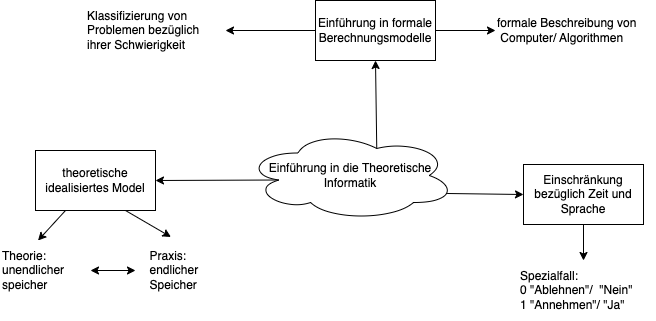
\includegraphics[width=1\textwidth]{Einführung.png}
    \caption{Überblick theoretische Informatik}
    \label{fig:example}
\end{figure}

% Rest of your document goes here...

\section{Grundlagen}

\subsection{Notationen und begriffe}
\begin{itemize}
    \item $\mathbb{N}$ bezeichnet die \{1, 2, 3\}
    \item $\mathbb{N}_{0}$, sei $[n]$ = \{1,$\ldots $,n\} und $[n]_{0}$ = \{0, 1, $\ldots $,n\} 
    \item Für eine Menge A und n$\in \mathbb{N}$ ist $A^{n}$ = \{($a_{1},\ldots, a_{n}$): $a_{1}$, $\ldots$ $a_{n}$ $\in$ A\}
    \item Für n $\in \mathbb{N}$ ist eine n-äre partielle funktion $\varphi$ : $A^{n} \leadsto B $ eine Funktion mit dom($\varphi$) $\supseteq A^{n}$ und Im($\varphi$) $\subseteq$ B. 
    Für $a_{1}$, ..., $a_{n}$ $\in$ A bedeuted $\varphi$($a_{1}$, ..., $a_{n}$)$\downarrow$, dass ($a_{1}$, ..., $a_{n}$) $\in$ dom($\varphi$) gilt und $\varphi$($a_{1}$, ..., $a_{n}$)$\uparrow$ bedeutet, 
    dass ($a_{1}$, ..., $a_{n}$) $\notin$ dom($\varphi$). Statt $\varphi$($a_{1}$, ..., $a_{n}$)$\uparrow$ schreiben wir auch $\varphi$($a_{1}$, ..., $a_{n}$) = $\uparrow$.
    Die partielle Funktion $\varphi$ ist total, wenn dom($\varphi$) = $A^{n}$ gilt.
    \item Eine lineare Ordnung, auch totale Ordnung, auf einer Menge A ist eine Relation $\leq  \subseteq  A^{n}$m sodass die folgende Eigenschaften erfüllt sind. 
    (wie für Relationen üblich verwenden wir hier Infixntation, schreiben also für a,b $\in$ A den Ausdruck a $\leq $ b anstatt (a,b) $\in \leq $ ): 
    \begin{enumerate}
        \item[(i)] a $\leq $ a $\forall$ a $\in$ A (Reflexivität)
        \item[(ii)] a $\leq $ b $ \land $ b $\leq $ a $\Rightarrow $ a = b $\forall$a,b $\in$ A (Antisymetrie)
        \item[(iii)] a $\leq $ b, b $\leq $ c $\Rightarrow$ a $\leq $ c $forall$a,b,c $\in$ A (Transitiität)
        \item[(iv)] a $\leq $ b $\vee$ b $\leq $ a $\forall$a,b $\in$ A (Totalität)
    \end{enumerate} 
\end{itemize}

\subsection{Alphabet, Wörter und Sprachen}
Eingaben und Ausgaben in unseren Berechnungsmodellen werden wörter genannt, wobei wir beliebige Zeichenketten als Wörter zulassen.

\subsection{Definition (Alphabet)}
Ein Alphabet ist eine nichtleere endliche Menge $\Sigma$. Das Alphabet $\Sigma$ wird $\lvert \Sigma \rvert$- är bezeichnet. Die Elemente von $\Sigma$ heißen Buchstaben oder Symbole.

\subsection{Definition (Wörter)}
Ein Wort über einem Alphabet $\Sigma$ ist eine endliche Folge von Symbolen aus $\Sigma$. Die Länge eines Wortes w ist $\lvert$w$\rvert$. Für i $\in\lvert$w$\rvert$ bezeichnet w(i) das i-te Element von w und für Symbole $a_{1}$, $\cdots$, $a_{n} \in \Sigma$ bezeichnet $a_{1}, \cdots, a_{n}$ das Wort w der Länge n mit w(i) das i-te Element von w und für Symbole $a_{1}, \cdots, a_{n} \in \Sigma$ bezeichnet $a_{1}$, $\cdots$, $a_{n}$ das Wort w der Länge n mit w(i) = $a_{i}$ $\forall$i$\in$ \([n]\). Das Wort der Länge 0 heißt leeres Wort und wird $\lambda$ bezeichnet. Ein Wort der länge 1 wird mit dem Symbol w(1) identifiziert.

\subsection{Definition (Binärwörter)}
Das Alphabet \{0, 1\} heißt Binäralphabet. Die Wörter über dem Binäralphabet heißen Binärwörter.

\subsection{Definition}
Die Menge Aller Wörter über $\Sigma$ wird mit $\Sigma^{*}$ bezeichnet. Für n $\in$ $\mathbb{N}_{0}$ setzen wir:
\begin{itemize}
    \item[] $\Sigma^{\leq n}$ := \{w $\in \Sigma^{*} : \lvert$w$\rvert \leq $n\}
    \item[] $\Sigma^{=n}$ := \{w $\in \Sigma^{*} : \lvert$w$\rvert = $n\}
    \item[] $\Sigma^{\geq n}$ := \{w $\in \Sigma^{*} : \lvert$w$\rvert \geq $n\}
    \item[] $\Sigma^{+}$ := $\Sigma^{\leq 1}$
\end{itemize}

\subsection{Definition (Verkettung)}
Für Wörter $w_{1}, w_{2}$ ist die verkettung  $w_{1} \circ w_{2}$, auch $w_{1}w_{2}$, von $w_{1}$ und $w_{2}$ ist definiert durch:
\[w_{1} \circ w_{2} := w_{1} \cdots w_{1} (\lvert w_{1} \rvert)w_{2} \cdots w_{2} (\lvert w_{2} \rvert)\]
Für ein Wort w und n $\in \mathbb{N}_{0}$ ist $w^{k}$ induktiv definiert durch $w^{n}$ := $\lambda$ falls n = 0 und $w^{n}$ := $w^{n-1} \circ w^{n}$ falls n $\geq $ 1. Für eine Sprachen $L_{1}$, $L_{2}$ sei durch $L_{1} \circ L_{1}$, auch $L_{1}L_{2}$ definiert durch
\[L_{1} \circ L_{1} := \{w_{1}w_{2} : w_{1} \in L_{1}, w_{2} \in L_{2}\}\]
Für eine Sprache L und 



\end{document}
